% FH Technikum Wien
% !TEX encoding = UTF-8 Unicode
%

\documentclass[MSC,Master,english]{twbook}%\documentclass[Bachelor,BMR,ngerman]{twbook}
\usepackage[utf8]{inputenc}
\usepackage[T1]{fontenc}
% BERND: Additional Pkg
\usepackage{tcolorbox}
\usepackage{xcolor}
\usepackage{hyperref}
\usepackage{listings}
\usepackage{graphicx}
\usepackage{amsmath}

\usepackage{amssymb}% http://ctan.org/pkg/amssymb
\usepackage{pifont}% http://ctan.org/pkg/pifont
\newcommand{\cmark}{\ding{51}}%
\newcommand{\xmark}{\ding{55}}%

\lstset{
    captionpos=b,
    numberbychapter=false,
    caption=\lstname,
    frame=single,
    rulecolor=\color{gray},
    numbers=none,
    stepnumber=1,
    numbersep=2pt,
    xleftmargin=15pt,
    framexleftmargin=15pt, 
    %umberstyle=\tiny,
    tabsize=3,
    columns=fixed,
    basicstyle={\fontfamily{pcr}\selectfont\footnotesize},
    keywordstyle=\bfseries,
    commentstyle={\color[gray]{0.33}\itshape},
    stringstyle=\color[gray]{0.25},
    breaklines,
    breakatwhitespace
}
\lstloadlanguages{bash}

% Define Code-Color
\definecolor{codegreen}{rgb}{0,0.6,0}
\definecolor{codegray}{rgb}{0.5,0.5,0.5}
\definecolor{codepurple}{rgb}{0.58,0,0.82}
\definecolor{backcolour}{rgb}{0.95,0.95,0.92}

% Bitte in der folgenden Zeile den Zitierstandard festlegen
%\newcommand{\FHTWCitationType}{IEEE}
%\ifthenelse{\equal{\FHTWCitationType}{HARVARD}}{\usepackage{harvard}}{\usepackage{bibgem}}
%BERND: TBH that package is 20 years old, get some more up2date packages for cite
\usepackage[utf8]{inputenc}
\usepackage[english]{babel}
\usepackage{csquotes}
%\usepackage[backend=biber,style=ieee,bibstyle=ieee]{biblatex}
%\usepackage[backend=bibtex,style=numeric,bibstyle=ieee]{biblatex}
%ARCH Linux fix
\usepackage[backend=biber,style=numeric,sortcites,natbib=true,sorting=none]{biblatex}
\addbibresource{Literatur.bib}


%Formatieren des Quellcodeverzeichnisses
\makeatletter
% Setzen der Bezeichnungen für das Quellcodeverzeichnis/Abkürzungsverzeichnis
%in Abhängigkeit von der eingestellten Sprache
\providecommand\listacroname{}
\@ifclasswith{twbook}{english}
{%
    \renewcommand\lstlistingname{Code}
    \renewcommand\lstlistlistingname{List of Code}
    \renewcommand\listacroname{List of Abbreviations}
}{%
    \renewcommand\lstlistingname{Quellcode}
    \renewcommand\lstlistlistingname{Quellcodeverzeichnis}
    \renewcommand\listacroname{Abkürzungsverzeichnis}
}
%Wenn die Option listof=entryprefix gewählt wurde, Definition des Entyprefixes für das
%Quellcodeverzeichnis. Definition des Macros listoflolentryname analog zu listoflofentryname und
%listoflotentryname der KOMA-Klasse
\@ifclasswith{scrbook}{listof=entryprefix}
{% 
    \newcommand\listoflolentryname\lstlistingname
}{%
}
\makeatother
\newcommand{\listofcode}{\phantomsection\lstlistoflistings}


%
% Einträge für Deckblatt, Kurzfassung, etc.
%
\title{Kubernetes on the Edge}
\author{Bernd KLAUS, BA}
\studentnumber{2010303012}
\supervisor{Dipl.-Ing. Hubert Kraut}
\secondsupervisor{Dipl.-Ing. Andreas Happe}
\place{Vienna}

\kurzfassung{
Kubernetes wird als Schweizer Armemesser der Container-Orchestrierung bezeichnet. Auch im Bereich edge-computing bietet der Dienst eine Vielzahl an unterschiedlichen Werkzeugen und Tools an, welche Teils unterschiedliche Strategien und Ansätze verfolgen. Die Auswahl reicht von einem zentralen Kubernetes-Cluster der verteilte Geräte, sogenannte „Leafs“, steuert bis hin zu vielen einzelnen und verteilten kleinen Clustern an der Edge, welche zentral gesteuert werden. Entscheidend ist es den richtigen Anwendungsfall zu erheben, um sich für die optimale Lösung entscheiden zu können. Ebenfalls spielen sicherheitstechnische Aspekte bei derart komplexen Umgebungen eine wichtige Rolle. Die vorliegende Arbeit gibt Einblicke und Entscheidungsgrundlagen sowie Empfehlungen hinsichtlich der IT-Security. Belegt werden die Angaben durch Implementierung eines Proof-of-Concepts
}
\schlagworte{Kubernetes, edge-computing, distributed System, Proof-of-Concept}


\outline{
Kubernetes is the de facto swiss-army-knife for orchestrating container-platforms. In addition, Kubernetes can also be used for deploying devices as well as applications on top of it on the edge of the network. However, there are different methods for archiving comparable results. On the one hand a possible solution is to build a central instance managing small distributed and independent clusters, on the other hand a centralized cluster with just leafs on the edge may be a better fit. This results in the challenge to find the best solution for the desired environment respectively use-case. The following thesis is making use of "Design Science Research" to give introductions on how to choose the proper architecture for the aimed environment.
}
\keywords{Kubernetes, edge-computing, geo-distribution, proof-of-concept}

%
% Start the Thesis
%

\begin{document}
\maketitle
\chapter{Introdutcion}
\label{chap:introduction}
Because of \ac{IoT} Devices becoming more and more common, the number of devices capable of communicating with the \ac{WWW} increases rapidly. Consequently, also the overall traffic generated as well the amount of data which must be processed increases accordingly. Regarding this development edge-computing is the rising start trying to solve that issues. Thereby data is not processed centrally like in traditional datacenters, but it is tried to handle those data close to the user within several distributed systems. Because of this methodology only really necessary data is transmitted to a central instance for further treatment and those the processing-power as well as the bandwidth necessary for processing required data is reduced significant. \par It is expected that the number of IoT devices will continue to grow fast \cite{SotE21} over the coming years. Concomitant edge-computing also will become more important in the future and become an important role in modern \ac{IT} architectures. \par To be able to control distributed systems effectively \ac{K8s} is providing a lot of useful tools and functions. Fundamentally there are two different approaches regrading the architecture of how to build an edge-computing environment making use of \ac{K8s}:

\begin{itemize}
    \label{item:architecture}
    \item \textbf{Default}: A centralized \ac{K8s} Cluster controlling many leaf-devices (workers) on the Edge.
    \item \textbf{Distributed}: Small and distributed \ac{K8s} Clusters running independent on the Edge controlled by a centralized Master-Instance.
\end{itemize}

Another upcoming approach of solving that issue is making use of the service mesh \cite{servicemesh}. This ultimately uses or builds on both of the aforementioned technologies. However, since this thesis concentrates on the two main architectures and their differentiation, the service mesh is not the main focus and just mentioned for the sake of completeness.

\section{Problem area}
Problems arise when trying to find the proper architecture for a specific use-case. There is no clear winner when comparing the above-mentioned different variants. Each of them  has their own pros and cons and may decide whether a project is successful or not. It is therefore all the more important to choose the proper architecture right before starting, changing the strategy in retrospect would take a lot of time and effort. However, there is no clear guidance on how to find the proper target environment, at least none which apply in general. Occasionally one finds recommendations for a very specific use case, however the chance is slim low this findings fit your goals respectively enlighten the decisions. This leads us to the following research question.

\section{Research question}
\label{sec:rq}
This paper is going to answer the subsequent research questions:
\begin{enumerate}
    \item What are the main differences of the in \autoref{item:architecture} mentioned architectures regarding functionality, scalability, costs and security?
    \item Which decision criteria must be defined respectively examined to create a catalog capable
    of choosing the proper architecture easier for \ac{IT} managers as well as administrators?
    \item Is there a trend in which technology is most likely to be used?
\end{enumerate}

\section{Goal}
\label{sec:goal}
The main goal of this thesis is to highlight the pros and cons for each of the \hyperref[item:architecture]{architectures} defined in the \hyperref[chap:introduction]{Introduction}. The focus will be mainly on the geo-distribution aspect. Although \ac{IoT} is playing a major role in pushing the development forward, however it is not considered further in the present work. To find the proper architecture, or at least recommendations what could fit best for different desired use-cases, a catalog will be defined. An important part will become the decision criteria catalogue helping people making comprehensible decisions based on scientific research. The main characteristics which are taken into account are scalability, state-of-the-art, handling, costs as well as security.

\section{Methodology}
\label{sec:methodology}
In the first part of the present work existing literature will be inspected. Related and relevant work will be examined accordingly and linked in the document. Also results will be incorporated to get out the most of it. The goal is to create a list with main criteria necessary for decision-making. As a result, a catalogue of criteria is drawn up in order to be able to decide on the right architecture. The \ac{DSR} method serves as a scientific method and to test the characteristics recorded in the catalogue. This chapter is given the most attention, it is the area where new techniques or architectural decisions are finally verified and the proof is given whether the catalogue works as expected or not. In the latter case, the catalog will be revised to reflect the findings of the last step and re-examined again using \ac{DSR}.


\chapter{State of the Art}
\label{chap:current}
\section{Technology}
The present chapter provides an introduction to the general thematic. The main components and objects of \ac{K8s} are explained aswell as the layers of edge-computing are highlighted. If anyone is already familiar with the subjects, may you jump over to the \autoref{sec:architecture} "architecture" to read further.
\label{sec:technology}
\subsection{Kubernetes}
To promote modern development and be able to implement continuous deployment pipelines cumbersome monolithic applications are divided into many smaller units. Each of these units provides only one function. In order to establish the overall functionality, these units are communicating with each other and thus provide services or make use of other ones. This new method of delivering applications brings many advantages in terms of development but also introduce some new challenges and complexities regarding operation. To simplify the tasks around the management of this architecture, \ac{K8s} has established itself as the de facto standard \cite{k8ssurv}. \ac{K8s} was initially developed by Google and later donated to the opensource community. Over the course of time, a broad community has developed around \ac{K8s} and a number of additional tools and extensions have emerged as a result. The most promising solutions regrading geo-distribution respectively edge-computing are highlighted in the subsequent \autoref{sec:architecture} "architecture". In order to be able to interpret the results of the use-cases, as well as building the necessary basic understanding, the following functionalities and components of \ac{K8s} are of relevance.  

\begin{figure}[ht]
    \centering
    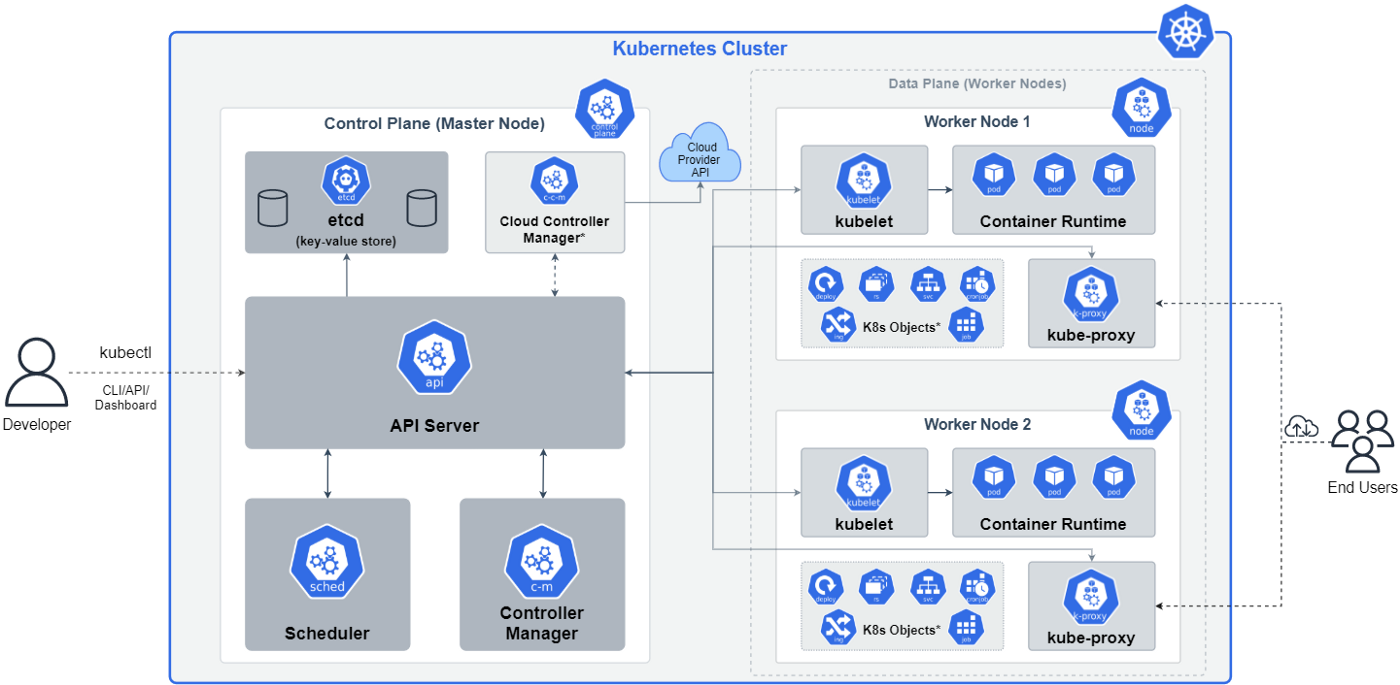
\includegraphics[width=0.75\textwidth]{PICs/k8s-architecture.png}
    \caption{\ac{K8s} architeture overview \cite{pic-k8s-overview}}
    \label{fig:k8s-architecture}
\end{figure}

\paragraph{Master Nodes} run the so-called \textit{Control Plane} which is responsible for controlling the cluster itself and all the ressources within. The Control Plane consist of the following components \cite{k8scomp}.
\begin{itemize}
    \item \textit{kube-apiserver} - acts as frontend web-interface responsible for controlling the \ac{K8s} cluster as well as the objects inside the cluster. Tools like kubectl abstract the \textit{OpenAPI v2} endpoint and provide access in form of a simply understandable and usable \ac{CLI}. 
    \item \textit{etcd} - represents a high-available and consistent key value store responsible for storing the actual state as well as the desired configuration of the cluster.
    \item \textit{kube-scheduler} - is responsible for scheduling pods on the available worker nodes. Decision variables such as available ressources, affinity-rules and constraints are taken into account. However, the default \textit{kube-scheduler} ist not aware of any latency between the worker nodes nor the pods communicating with each other. As discovered in the following chapters, this appears to be an important variable for edge-deployments. However, some available white-papers already try to address those issues and show possible solutions by adopting a custom scheduler taking care of those values. More details on this can be found in the \autoref{chap:related} "related work".
    \item \textit{kube-controller-manager} - consists of a single compiled binary controling the status of nodes, jobs, service-accounts and endpoints as well as creating or removing them.
    \item \textit{cloud-controller-manager} - represents the interface to the underlying cloud-platform. This allows kubernetes to create and/or configure load-balancers, routes and persistent-volumes on the underlying cloud-infrastructure. In a local environment e.g. minikube \cite{minikube} provide the \textit{cloud-controller-manager} - becomes an optional component and is not required. The same may apply to edge-locations as those areas are outside the cloud most of the time.
\end{itemize}

\paragraph{Worker Nodes} manage the workload, i.e. run the actual application(s). These nodes are composed of the following, see list below, parts \cite{k8scomp}. It should be mentioned, that also the described \textit{Master Nodes} are executing those components because some core-componentes are containerized (pods) itself. 
\begin{itemize}
    \item \textit{kubelet} - is an agent which assures that the container is executed properly inside their associated pods according to its specifications defined via \textit{PodSpec}. Also \textit{kubelet} is responsible for monitoring the healthy state of the containers.
    \item \textit{kube-proxy} - uses the packet filters of the operating system underneath to forward traffic to the desired destination. The resulting access points, also called \textit{Services} in \ac{K8s}-jargon, can be made available either internally or externally.
    \item \textit{container runtime} - is the part that finally executes the containers. The default runtime at time of writing is \textit{containerd}, however any runtime is supported that complies with the CRI specification \cite{cri-runtime}.
\end{itemize}

\paragraph{Kubernetes Objects} are persistent properties inside the \ac{K8s} ecosystem representing the state of a cluster. The most important feature of those objects is to describe the target environment in a declarative way. For this purpose, most of the time, YAML files are used. Kubernetes now ensures that the desired state of the environment is actually achieved and continuously monitors the required objects to meet those defined requirements. This mechanism is also ideal for distributed systems, such as edge computing, as availability can be monitored at any time and a an action can be taken if necessary. Subsequent the main objects are cited starting with the smallest unit \cite{k8sconc}.
\begin{itemize}
    \item \textit{Containers} - decouple the actual application and its dependencies from the underlying infrastructure. The main properties of those containers are there immutability and repeatability. This means that the container can be rebuilt at anytime resulting in an identical clone. Likewise, the code of a running container cannot be modified subsequently.
    \item \textit{Pods} include at least one or more \textit{Containers}. In the most scenarios a single pod consists of a single container, in some cases a so-called sidecar container is used increasing the number of containers inside a pod. Containers which are in the same \textit{Pod} share the same local Socks as well as volumes mounted.
    \item \textit{Deployments}, \textit{Statefulsets} and \textit{Daemonsets} - are responsible for ensuring the actual workload is provided, to achieve this they control and scale the assigned \textit{Pods}. When creating an application for \ac{K8s}, it is most likely to create one of those objects. The \textit{Pods} and \textit{Containers} are merely an end product that is derived these objects.
    \item \textit{Services} - provide an abstract way to make a set of \textit{Pods} available on the network via a single endpoint. Additional deployed pods will automatically be added to the responsible \textit{Services}. Thereby \ac{K8s} is an excellent choice when it comes to scaling applications without any manual intervention. This also applies for deploying applications to the edge of the network, as illuminated in the course of this thesis. Closely related to the \textit{Services} - is the \textit{Ingress} resource, which is taking care of making the aforementioned objects available outside the cluster. An optional reverse-proxy (\textit{Ingress-Controller}) must be installed in order to make use of the latter. \newline
    A new feature, which is of relevance regarding edge-computing, currently in beta phase, is the so-called \textit{Topology Aware Hint}. Basically its meta-data added to the endpoints defined previously suggesting the connection client on how to reach the destination efficiently (e.g. zones aware of different locations can be defined)
    \item \textit{ConfigMaps} and \textit{Secrets} - are pieces of information which can be mounted into to \textit{Container} to adjust the configuration inside at runtime. Even whole files can be replaced using on of them. \textit{Secrets} are only different in the sense that they decode the content, however technically they are the same.
    \item \textit{Volumes} - provide persistent storage which extends beyond the life cycle of the pods. Volumes can be mounted at any defined position inside the pods. The disadvantage is that the data written to those \textit{Volumes} resides out of the \ac{K8s} ecosystem and therefore the operator must take care of data security and replication. This becomes even more complicated in an edge-computing environment where nodes have higher latency between them.
\end{itemize}

\subsection{Edge-Computing}
Edge-computing is the model that extends cloud services to the edge of the
network. The computing resources on the edge act as a layer between the user, who provides or wants to process data, and the centralized datacenter (e.g. the cloud). Because data can be processed earlier respective closer to the source, latency and amount of data transferred can be reduced \cite{intro-edge}. Also, the required computing-ressources in the datacenter can be minimized because data can be processed at the edge. A major driver of the subsequent s technology is \ac{IoT}. The amount of devices and resulting data volume, which must be processed, is increasing exponentially \cite{SotE21}. Another technology which depends on it are low-latency applications like e.g. video-streaming. 

\paragraph{Hierarchy} descripes the layers of the architecture. The following list enumerates the most important layers from top to bottom \cite{intro-edge}.
\begin{enumerate}
    \item \textit{Cloud} - centralized datacenter
    \item \textit{Fog} - distributed "smaller" datacenters
    \item \textit{Edge} - the closest unit to the end-user
    \item \textit{\ac{IoT}} - device at the edge put into use
\end{enumerate}


The main focus of this work is to efficiently combine the two layers \textit{Cloud} and \textit{Edge} and orchestrate between them using \ac{K8s}. The layer \textit{Fog} is skipped because it is often seen to be "the same" as the \textit{Edge}. Also, current \ac{K8s} based solutions do not make use of it. 

\paragraph{Geo-Distribution} characterises the aspect of the geographical propagation of the edge ressources. The goal is to provide computing power over wide areas, each close to the users. By establishing many of these locations in different regions, network latency can be significantly reduced from the user's perspective. However, the latency between the edge-nodes and the centralized cloud still remain.


\section{Architecture}
\label{sec:architecture}
This chapter focuses on the two different architecture approaches which can be used for edge computing. After an overview the advantages and disadvantages as well as possible solutions are examinated.

\subsection{Default}
\label{sec:arch-default}
In order to be able to manage resources at the edge, a traditional architecture can be used. This is subdivided into a centralized control plane hosted in the cloud and distributed worker nodes near the edge. The same \ac{K8s} architeture is commonly used when deploying to a single location aswell inside the cloud. The following graphic illustrates the architecture.

\begin{figure}[ht]
    \centering
    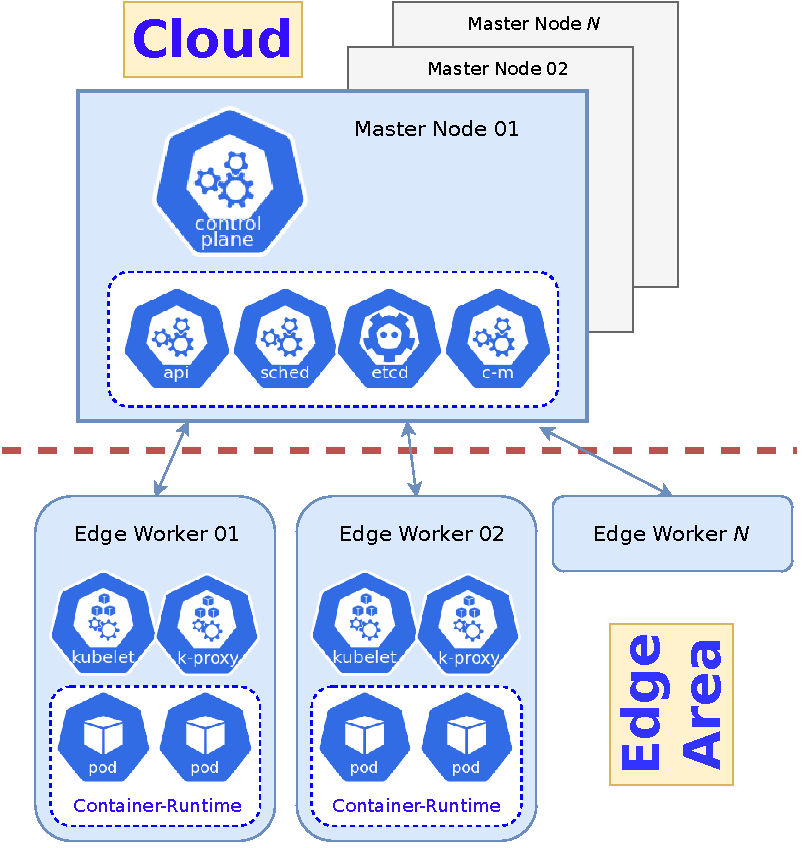
\includegraphics[width=0.60\textwidth]{PICs/drawio/defaul-k8s.drawio.pdf}
    \caption{Default \ac{K8s} architeture}
    \label{fig:k8s-default}
\end{figure}

Although the conventional components can also communicate with each other over long distances, there are still some challenges that need to be taken into account. An important role in this context is played by the \ac{CNI}. This part of \ac{K8s}, which can be selected in the form of a plugin, is responsible for the cluster-internal network traffic. Most of these plugin providers offer advanced features that facilitate geographical distribution. Some of the most used \ac{CNI} providers are \cite{k8s-cni}:

\begin{itemize}
    \itemsep0em
    \item Calico
    \item Canal
    \item Cilium
    \item Flannel
    \item Weave
\end{itemize}

Other issues, which must be observed, are the replication of metadata hold by the control planes. Because of the higher latency and-or unstable connection at the edge site data may cannot always be reliably retrieved. To circumvent this problem, asynchronous replication can be used for replicating metadata. Another solution is to make independent, thereby no big data chunks are requested at all. The important part of the metadata store are \ac{DNS} entries, because \ac{K8s} heavily relies on them for service discovery. NodeLocal DNS is the recommand way \cite{k8sdnslocal} to hold a copy on the worker nodes. 

Another challenge regarding storage ist the handling of persistent volumes. Those logical data chunks must be replicated in an asynchronous manner because of the latency between the nodes. As this is not alway possible and data management is a generel challenge, making services stateless is the recommand way to work arround this issue.  In contrast to this, forwarding data to the cloud is not an issue in most of the times when using suitable message queues. For that purpose, eg. KubeEdge, is making use of \ac{MQTT}.   

In addition there is no awarness of where workloads are running and the level of latency between nodes when using vanilla kubernetes. There are some developments in this area, but they have not really caught on yet \cite{k8s-sharping-edge}\cite{tk-k8s-edge-scheduler}\cite{5g-k8s-scheduler}.

\paragraph{KubeEdge} is an open-source \ac{CNCF} project \cite{hal-kubeedge} that already comes with many of these functions respectively requirements pre-charged. Likewise, this tool was explicit developt for edge-computing.  Worker nodes can therefore be distributed across the hole globe without any major adjustments. To make this possible, some components were added or exchanged \cite{kubedge}.

\begin{itemize}
    \item \textit{CloudHub} - webSocket endpoint responsible for sending data to the edge-nodes.
    \item \textit{Edged} - kubelet is replaced with a lightweight custom agent, the EdgeCore. Thereby also devices with very limited ressources, e.g. a Raspberry Pi, can be used for running workloads.
    \item \textit{EdgeController} - a \ac{K8s} controller responsible for managing and distributing metadata.
    \item \textit{EdgeHub} - the counterpart to the Edgecontroller; uses a websocket server for syning updates to and from the cloud.
    \item \textit{MetaManager} - Message processor, coordinating between edgehub and edged. Can also store information in an SQLite database. In case of connectivity issues those database is used so that services can continue to run continuously.
    \item \textit{EdgeMesh} - responsible for replacing the \ac{K8s} default network functionalities such as the kube-proxy, \ac{DNS} and \ac{CNI} and making them fit for edge scenarios. Main goal was to achieve high availability, reliability and the agent as lightweight as possible. However, this agent also has some disadvantages, as we will discover in the use-cases later. It should also be mentioned that this agent is not installed per default and is being developed in a separate project.
\end{itemize}

The following graphic illustrates the interaction of the components. 
\begin{figure}[ht]
    \centering
    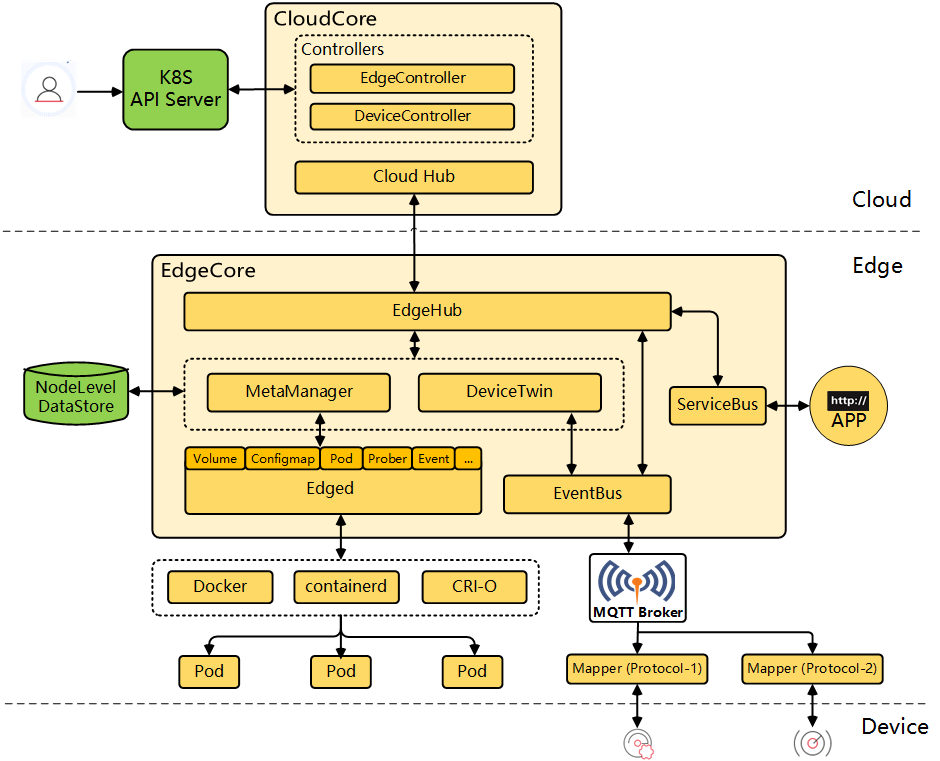
\includegraphics[width=0.70\textwidth]{PICs/kubeedge-arch.png}
    \caption{KubeEdge architecture\cite{ke-docs-why}}
    \label{fig:ke-architecture}
\end{figure}

In addition a component (EventBus) for device management and seemles integration with \ac{MQTT} is built-in to KubeEdge\cite{hal-kubeedge}. However, because this thesis focuses on the geo-distribution aspect, this part is not researched further.


\subsection{Distributed K8s}
\label{sec:disk8s}
In this case, a different approach is chosen and, in contrast to the previous architecture, fully-fledged clusters are also operated at the edge. The obvious advantage is that they can be operated autonomously. There is basically no dependence on the other nodes or there workloads.

\begin{figure}[ht]
    \centering
    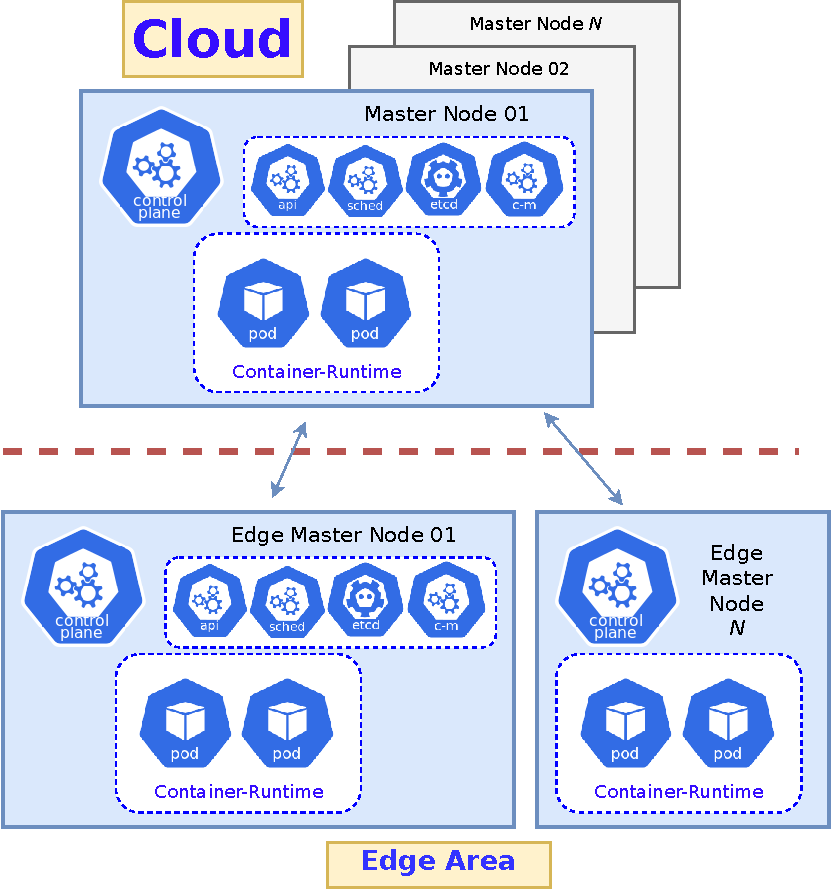
\includegraphics[width=0.60\textwidth]{PICs/drawio/distributed-k8s.drawio.pdf}
    \caption{Distributed \ac{K8s} architeture}
    \label{fig:distributed-k8s}
\end{figure}

However, this also creates new challenges such as the distribution and coordination of workloads. Without additional functionality added, the workload running on the clusters does not know about their neighbours. To overcome this gap, the division  "multi-cluster deployment" has excelled in recent years. Even Google, the original developer of \ac{K8s}, offers such a service \cite{google-mcs} in their public cloud. Due to the increased demand, the \ac{KubeFed} tool is officially being maintained and further developed by the \ac{K8s} project\cite{kubefed-github}. Although the tool is still in beta, it is a very good choice for our field of application. One possible alternative would be the \ac{K8s} manager by Rancher Labs.

\paragraph{\ac{KubeFed}} consists of a central hosting cluster which controls subordinate clusters via \ac{API} delegation. Within \ac{KubeFed} you can define which configuration should be managed by the hosting cluster. The methodes used are intentionally low-level and can thus be expanded well for different edge-deployment variants. Two different types of information is used to configure \ac{KubeFed}\cite{kubefed-github}:

\begin{itemize}
    \item \textit{Type configuration} - determines which \ac{API} types are handeld.
    \item \textit{Cluster configuration} - determines which clusters should be targeted.
\end{itemize}

The type configuration itself consist of three main parts:

\begin{itemize}
    \item \textit{Temaplates} - defines a reprenentation of common ressources across the clusters.
    \item \textit{Placement} - defines which destination-cluster the workload should run on.
    \item \textit{Overrides} - defines varation of the templates on a per cluster level.
\end{itemize}

One disadvantage of KubeFed is the lack of network integration. Workloads running on distributed clusters cannot communicate with their neighbours. The integration of the standard CNIs listed above is not possible. However, additional components or configurations can now also solve this problem, as Cilium demonstrates \cite{ciliummesh}. However, since this paper focuses on the comparison of the two architectures themselves, such extensions are not considered.

\section{General Challenges} 
\label{sec:generalchallanges}
Challenges that appear when creating respectively operating such infrastructures are diverse, as can be seen in the following list \cite{intro-edge}.

\begin{itemize}
    \item \textit{Variety} - a lot of different locations, technologies as well as methods on how to control devices on the edge is challenging for both development and operation. The better these different factors can be abstracted and simplified, the more effectively the infrastructure can be used.
    \item \textit{Integration} - edge-computing evolves very quickly, thereby things could change quickly. The more important it is to keep the provided interfaces extensible. This way, new devices or application can be put in use swiftly. 
    \item \textit{Awareness} - the devices and/or end-user do not care about how their traffic is routed, or their data is processed. However, the architecture needs to take care of that to use the topology in the best possible way.
    \item \textit{Resources} - scaling Resources like \ac{CPU}, \ac{RAM} and disk space at the edge is by far more elaborate than in a datacenter or in the cloud.
    \item \textit{\ac{QoS}} - The service provided at the edge should be reliable and provide a good user experience. Availability and performance play a central role in this context. As the availability can not be guaranteed to some extent, an appropriate failover mechanism should be in place.
    \item \textit{Security} - physical access control as well as isolating applications from each other is a difficult task. Also, the data traffic must be separated accordingly. In general, \ac{IT} security is a hot topic, and especially at the edge, it requires appropriate consideration for hardening the environment.
    \item \textit{Monitoring} - another important factor is how to capture metrics and events (logs) from the edge. They need to be indexed on a centralized instance in order to get a general overview on what's happening. Because of the dynamic and rapid changes some kind of automatic discovery should be used for that purpose.
    \item \textit{Environment} - Some locations may have to deal with difficult conditions regarding their surroundings. Increased dust exposure, poor internet connections or recurring power outages can be some of these factors. The system must be able to cushion or parry such failures accordingly.
\end{itemize}
The above-mentioned challenges provide a good starting point for defining the necessary tests to find the matching target architecture. Details about this test can be found in the \autoref{sec:dsrmethode} "methodlogy".



\chapter{Design Science Research}
\label{chap:dsr}
"A common topic when performing research in technical disciplines is to design some kind of artefact, such as a model, an information system, or a method for performing a certain task. To address this topic in a systematic and scientific way, Design Science Research (DSR) has stablished itself as an appropriate research method." \cite{dsr-method}

\section{Methodology}
\label{sec:dsrmethode}
According to the description in the introduction before, \ac{DSR} is used as a scientific method to construct the \ac{PoC}. For this purpose two real world exmaples are build, which are then gradually refined. Those exmaples are descripte in detail in the following \autoref{sec:dsrenv} "environment". The same \hyperref[sec:dsrusecase] are then deployed onto each of these environments. Afterwards, Tests are then defined and carried out on the basis of the issues listed in section \autoref{sec:generalchallanges} "genereal challenges". Based on the results, a preferred environment per property can finally be determined.

\section{Environment}
\label{sec:dsrenv}
\subsection{Generel}
The main goal is to create both of the aimed architectures in a similar environment. The target environment should provide good coverage of the diversity encountered in edge environments. For that poropse the \ac{PoC} is build across \hyperref{https://www.hetzner.com/cloud}{}{}{Hetzner Cloud} and a local site connected via 4G mobile internet.

\paragraph{Coverage} This combination allows a wide range of possibilities to be achieved:

\begin{itemize}
    \item \textit{Geographical distribution} - Hetzner Cloud offers location in Germany, Finland and the U.S for deployments. This allows communication to take place over long distances.
    \item \textit{Scalability} - On the Hetzner Cloud scaling nodes can be realised quickly via \ac{API}.
    \item \textit{\ac{NAT}} - At the local site, nearby vienna, no public IP is availabe for each of the nodes. Therefore, \ac{NAT} is used to map a dynamic changing IP to the nodes downstream.
    \item \textit{\ac{ARM}} - Also at the local site, a Raspberry Pi is used as an edge-node to emulate devices with minial ressources.
    \item \textit{Unstable} - The connection at the local site may be unstable from time to time because the connection is established over the public 4G network using mobile technology.
\end{itemize}

\paragraph{Locations} Subsequent, a tabular lists all of the nodes that are used for each of the both test environments, followed by a graphic showing the locations on a map.

\begin{table}[ht]
    \begin{center}
        \begin{tabular}{|l|l|l|l|l|l|l|}
            \hline
            Node & Location & IP & CPU & Cores & RAM & Latency \\
            \hline
            Master & Nürnberg, DE & dedicated & AMD64 & 2 & 4GB & 0ms \\
            Edge-1 & Ashburn, US & dedicated & AMD64 & 2 & 2GB & 95ms \\
            Edge-2 & Helsinki, FI &  dedicated & AMD64 & 2 & 2GB & 24ms \\
            Raspberry & Kirchberg, AT & dynamic & ARM64 & 4 & 4GB & 40ms \\
            \hline
        \end{tabular}
        \caption{\ac{PoC} nodes specification}
        \label{tab:poc-nodes}
    \end{center}
\end{table}

\begin{figure}[ht]
    \centering
    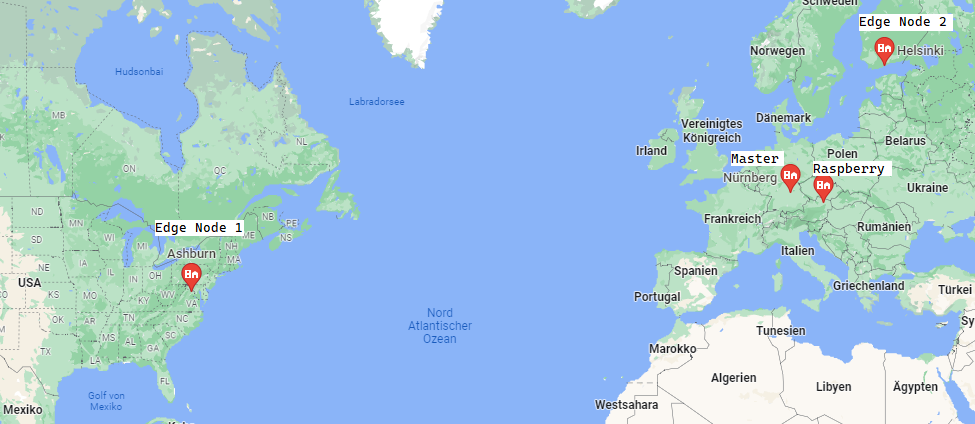
\includegraphics[width=0.80\textwidth]{PICs/poc-map.png}
    \caption{Map of the \ac{PoC}\cite{googlemaps}}
    \label{fig:poc-map}
\end{figure}

\paragraph{OS} The \ac{OS} used on all cloud nodes is Ubuntu 20.04.3 LTS. For the local site on the Raspberry Pi the \ac{OS} Raspberry Pi Lite, without \ac{GUI}, is used.

\paragraph{\ac{K8s}} For simplicity, the tool of choice for installing \ac{K8s} is \hyperref{https://k3s.io/}{}{}{K3s}. This is a lightweight \ac{K8s} distribution optimized for \ac{IoT} and deployments at the edge. All necessary features are supported, only the dependencies have been reduced to the essentials. In actual use, insofar as resources in the cloud only play a subordinate role, the standard \ac{K8s} can also be used analogously. However, at the edge K3s if a perfect match. To illustrate the simplicity, the installation command used is shown below.  

\begin{lstlisting}[caption={K3s installation},captionpos=b]
curl -sfL https://get.k3s.io | INSTALL_K3S_EXEC="--disable traefik --disable-cloud-controller" sh -s -
\end{lstlisting}

\paragraph{VPN} No \ac{VPN} is used for either environment. Although a VPN can increase security accordingly and services can communicate more easily, its use in a widely distributed edge environment with many nodes is problematic in most cases. Traditional VPNs are not designed for unstable connections with high latency and possibly rapidly changing \ac{IP} addresses. The tools used in both architetures therefore use alternative approaches via HTTPs and RPC respectively.

\subsection{KubeEdge}
\label{sec:dsrenvke}
For the default architecture resrespectively KubeEdge variant, only a \ac{K8s} installation on the master node is required. Edge nodes just need be to equipped with a supported containter runtime of choice. In our specific \ac{PoC} Docker is used. KubeEdge takes over the roles of the kublete and the kube-proxy as shown in the figure \hyperref[fig:k8s-default]{"default K8s architecture"}. A single binary (keadm) is used to initialise KubeEdge. A token and the public IP are specified as parameters on the master. On the edge nodes, those information is used to join the master. 

\paragraph{Challenges} The most important steps and challenges encountered during the installation are listed below.

\begin{itemize}
    \item \textit{CloudStream} - While the standard installation can be done easily, activating logs is much more challenging. Activities such as generating certificates, setting environment vairables and adapting configuration files must be carried out manually.
\end{itemize}

\paragraph{Installation} Steps for installation can be founf in the Github repository: \hyperref{https://github.com/Berndinox/K8sEdge/blob/main/DOCs/kubeedge-install.md}{}{}{Berndinox/K8sEdge}

\subsection{KubeFed}
\label{sec:dsrenvkf}
In contrast to KubeEdge, as also noted in \autoref{sec:disk8s}, KubeFed relies on individually acting clusters that are controlled by a central instance. Because of this, each node must be equipped with a fully functional \ac{K8s} cluster. Usually, the installation is associated with greater effort, but K3s simplifies this process enormously, as descripted in \autoref{sec:dsrenv}. 

\paragraph{Challenges} The most important steps and challenges encountered during the installation are listed below.

\begin{itemize}
    \item \textit{Hosting Cluster} - The challenges arise when it comes to connecting all instances from the central cluster. The kubeconfig for each of them must be modified, to include the puclic ip or \ac{FQDN} of the node, and transmitted to the central hosting cluster. There, the configuration must be added as an additional context. Finally, a custom binary is used to add each of the defined contexts to \ac{KubeFed}, as shown below.

    \begin{lstlisting}[caption={KubeFed join context},captionpos=b]
    kubefedctl join edge1 --cluster-context edge1 --host-cluster-context default --v=2
    \end{lstlisting}

    \item \textit{Dynamic IP} - Because the central hosting cluster is initialising the connection to the  nodes at the edge, these nodes must be reachable over a static adress. In most cases the use of static ips is not a problem. However, especially in edge-environments, the use of dynamic ip-addresses may be necessary. To circumvent this problem, a so-called dynamic \ac{DNS} service is used to establish the connection. Although such a service can be set up relatively quickly, it does mean that an additional component has to be installed and maintained. In contrast, \hyperref[sec:dsrenvke]{KubeEdge} works without such a workaround.
    
    \item \textit{dNAT} - As long as the target node is behind a router and connected with a private ip, destination \ac{NAT} must be configured to forward the necessary port. Alternatively, a reverse-proxy can be used to publish the internal service. This step is also only required for the KubeFed variant. 
\end{itemize}
\paragraph{Installation} Steps for installation can be founf in the Github repository: \hyperref{https://github.com/Berndinox/K8sEdge/blob/main/DOCs/kubefed-install.md}{}{}{Berndinox/K8sEdge}

\section{Use-Case}
\label{sec:dsrusecase}
\label{sec:dsrusecaseweb}
As a test, a web-application is distributed over several egde-nodes which is to be made accessible locally as well as via ClusterIP. The goal here is not to develop a complex application, but to uncover the behaviour of the environments. A ready-made nginx container, which is available for both arm and x86, is used as the test pod. The name of the docker image, available in the DockerHub, is: nginxdemos/hello. The \ac{K8s} objects used are composed of a service definition and a deployment file. The most important parts are listed here:

\begin{lstlisting}[caption={Web-application code},captionpos=b]
kind: Deployment
spec:
  selector:
    matchLabels:
      app: nginx1
    spec:
      containers:
      - image: nginxdemos/hello
        ports:
        - containerPort: 80
---
kind: Service
spec:
  ports:
  - name: http
    port: 8000
    targetPort: 80
  selector:
    app: nginx1
\end{lstlisting}

It is important to note that the above configuration only contains parts to increase readability and cannot be applied in this form. The full configuration can be found in the Github repository under the folder \hyperref{https://github.com/Berndinox/K8sEdge/blob/main/DOCs/}{}{}{DOCs}.

\subsection{KubeEdge} 
Starting the web-application on KubeEdge environment is not as simple as assumed. If the deployment and the service definition are created via kubectl, this looks quite successful at first. The service is created and pods are scheduled accordingly. However, our goal was to make the service-ip accessible from within the nodes of the cluster via ClusterIP. But, when the service is called via curl, an error appears. Another problem is that the pod cannot be accessed either directly on the exposed port or via kubectl exec.

After some research, it turned out that KubeEdge does not use any CNI plugin to offer network-connectivity per default. However, a specially developed Kube-API endpoint is used for this, which is to take over the functionalities and improve them for the requirements of an edge environment. This endpoint does not currently cover all functionalities, which is why our deployment needs to be modified accordingly \cite{ke-ake-gh}.

The following list represents the available Kube-API verbs:
\begin{itemize}
    \itemsep0em 
    \item Get
    \item List
    \item Watch
    \item Create
    \item Update
    \item Patch
\end{itemize}

Not implemented at time of writing is the verb \textbf{"Proxy"}, which prevents us from connecting directly to the pod via kubectl exec. Ohter commands that rely on the proxy verb are attach, top,  and logs. For the latter, there is already a solution in the official documentation, also noted in the code base of this thesis.\medbreak

Three variants are available to solve the problem of missing network connectivity.
\begin{itemize}
    \item \textit{Without network} - the first approach is to simply omit the network part and make your delpoyment independent of each other. However, this means that the actual added value of the \hyperref[sec:arch-default]{default architecture} is lost; the cluster no longer behaves like a location-bound cluster. Also the desccription found in the docs of KubeEdge seem not be be very accurate, when not using additional tools: "With KubeEdge, users can orchestrate apps, manage devices and monitor app and device status on Edge nodes just like a traditional Kubernetes cluster in the Cloud." \cite{ke-docs-why}
    \item \textit{CNI} - the next logical step seems to use a \ac{CNI}, which would make all the required functionalities available. However, this means that many of the advantages promised by KubeEdge are gone: The support of private-ip addresses behind \ac{NAT}, high availability and resilience as well as latency-independencie. In addition, a developer from KubeEdge points out that making use of a \ac{CNI} is not a recommand solution \cite{ke-cni-no}.
    \item \textit{EdgeMesh} - as described in \autoref{sec:arch-default} is an additional component which has to be installed manually. Although EdgeMesh is part of KubeEdge and integrates seamlessly, it is seen as a separate project whose development is independent. The addon promises to solve many of our problems and the supported functions seem optimal, but one should keep in mind that the project is still very young and only four releases have been issued.
\end{itemize}
In the course of solving the problem, two variants were examined in detail, firstly the one that does without all additional tools and secondly the variant with EdgeMesh. The variant with post-installed CNI is not considered further; in this case, one could fall back directly on vanilla \ac{K8s}.

\paragraph{Without network} As long as there is no need for complex network communication between the pods, this variant offers a simple solution. Deployments, StatefullSets and DaemonSets can be distributed and scheduled via \ac{K8s} to the edge-nodes. The services can then be made available for local services only. This is achieved through the configuration of a so-called HostPort. It is important to note that making the port available cannot be done via NodePort, as in this case the port would be made accessible at all nodes, which in turn requires a functioning cluster network. The following is the modified deployment that makes the application accessible on the edge-location. Please note that the object service was removed entierly, only relevant parts are cited.
\begin{lstlisting}[caption={Web-application HostPort },captionpos=b]
    spec:
      hostNetwork: true
      containers:
      - image: nginxdemos/hello
        ports:
        - containerPort: 80
        - hostPort: 8000
\end{lstlisting}

One possibility to establish the connection between the edge-locations in this variant would be the exchange via MQTT on the application level via the cloud component. However, this increases the complexity tremendous. In this case, one of the other two solutions is to be preferred at the current state of affairs.

\paragraph{EdgeMesh} As already noted, this component must be installed before it can be used. Before the actual installation, which takes place within the \ac{K8s} system, the KubeEdge configuration must be adapted. The installation is divided into the following steps.

\begin{enumerate}
    \item \textit{Load} - Download the EdgeMesh sources from Github
    \item \textit{CRDs} - Create the \ac{CRD} necessary
    \item \textit{KubeEdge} - Konfigure KubeEdg components
    \item \textit{Agent} - Apply the YAMLs provided by EdgeMesh
    \item \textit{Restart} - and verify your system-changes.
\end{enumerate}

The complete process is available in the following document: \hyperref{https://github.com/Berndinox/K8sEdge/blob/main/DOCs/kubeedge-edgemesh.md}{}{}{Berndinox/K8sEdge}. Please note that the project may change rapidly, the installation-process linked above is just a snapshot of the current state.  As long as EdgeMesh could be installed without errors, the deployment and service object described above can be distributed and scheduled without any modification. With this solution, the native \ac{K8s} approach is fully followed and ensured.\medbreak

What is certain is that the documentation at this point is not sufficiently well formulated. It advertises native \ac{K8s} support, which cannot be met with a default KubeEdge installation. Although it is pointed out that logging has to be configured separately, the networking section receives little or no attention. It was only through intensive testing and tracking of issues on Github that the above behaviour regarding connectivity could be uncovered. This fact is taken into account in the later evaluation.

\subsection{KubeFed} In principle, the same considerations must be made for delpoying on KubeFed as for those on KubeEdge without network support. The application must be designed so that no communication can take place between the clusters. However, the native approach of \ac{K8s} can be followed within the respective clusters at the edge. It would also be possible to operate several nodes at the respective edge-locations in the form of a cluster. Within this cluster, communication between the workloads would be possible without restrictions. Due to these properties, KubeFed is always particularly suitable when fewer and better developed locations are to be connected, which must be able to act independently. In order to roll out the deployment mentioned in the introduction of the chapter to the federated clusters, some adaptations are nevertheless necessary, which are illustrated below. 

\begin{enumerate}
    \item \textit{Enable API-Ressource} - On the master instance, the ressources earmarked for distribution must be enabled. Per-default KubeFed does not distribute any ressources. In this specific case, we have to enable the deployment and serivce object as follows.
    \begin{lstlisting}[caption={Enable federation},captionpos=b]
        kubefedctl enable deployments.apps, services --kubefed-namespace kube-federation-system
    \end{lstlisting}
    \item \textit{Create Namespace} - The first step is to create a namespace at the master, which then contains all the resources that are distributed to the clusters at the edge. In our first spefici use-case the namespace ist called "test1".
    \item \textit{Create Ressources} - At this point it is crucial to understand that KubeFed distinguishes between two types of objects. The normal objects, which are however only executed and managed on the master, and specially federated objects which will be deployed on the edge-clusters. The subsequent picture illustrates the interaction.
    \begin{figure}[ht]
        \centering
        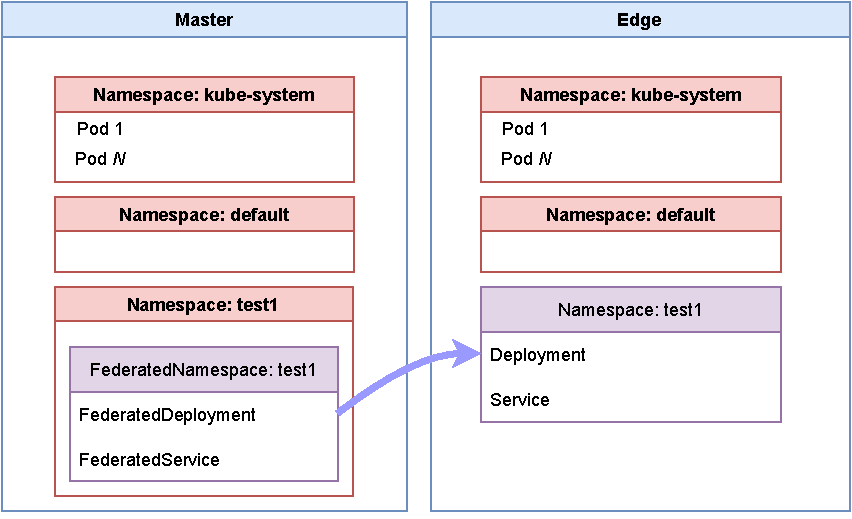
\includegraphics[width=0.70\textwidth]{PICs/drawio/kubefed-ressources.drawio.pdf}
        \caption{KubeFed objects}
        \label{fig:kubefed-ressources}
    \end{figure} \medbreak
    The conventional objects are simply preceded by the abbreviation "Federation". If the API-resource is also delegated, the objects are passed to the edge-clusters and schedulded there in form of the default objects. The environment at the edge does not even know about the existence of these special federated resources, because they are scheduld in form of a default object. The service and deployment mentioned at the beginning is therefore expanded as follows.
    \begin{lstlisting}[float,caption={Federated Object},captionpos=b]
        apiVersion: types.kubefed.io/v1beta1
        kind: FederatedDeployment
        spec:
          ...
        placement:
          clusters:
          - name: edge1
          - name: edge2
    \end{lstlisting}
    The same approach applies for the service object. An important part of the configuration is the placement part, which defines on which edge clusters the respective object is to be created. The complete configuration, can be found in following file saved on: \hyperref{https://github.com/Berndinox/K8sEdge/blob/main/DOCs/kubefed-usecase1.md}{}{}{Berndinox/K8sEdge}.
\end{enumerate}

\section{Performed Tests}
In addition to the previously described feasibility, the operation of the respective environment is also of great importance. In the following section, tests are therefore carried out on connectivity, resource utilisation and the application itself. If problems arise or environments do not function as expected, adjustments can be made in accordance with DSR guidelines. These adjustments are documented and described accordingly and can be regarded as best-practice.
\subsection{Ressource usage}
\label{sec:dsrtestress}
As already described in the \autoref{sec:generalchallanges}, the efficient use of resources is an important characteristic in the edge-computing environment. Due to the fact that we rely on K3s as \ac{K8s} distribution for the expression with KubeFed, which is known for using few resources, comparable results can be expected. In principle, however, KubeEdge should be somewhat more lightweight, since only a \ac{CNI} is used without full \ac{K8s} distribution. The only unknown is the deployment of EdgeMesh which could increase the resource requirements. The tests are performaned on the edge-side choosing node "edge-1" located in US. The uptime of the nodes for both environments, at time of the measurements, is exactly the same, approximately 15 minutes.

\subsubsection{Idle}
The first parameter to be considered is the CPU and Memory load while system is idle or under no significant load. The first test is carried out using the tool cpustat. "Cpustat  is  a  program  that dumps the CPU utilization of current running tasks (that is, processes or kernel threads).  cpustat is useful to monitor the  activity  of  long  lived processes in a system, such as daemons, kernel threads as well as typical user processes" \cite{cpustat}. \medbreak

\paragraph{CPU} The deployment created in the usecase is scaled to one pod per node, then the first measurement is performed in idle mode using the command: \lstinline|cpustat -x -D -a 1 30 -r export.csv|.
The utilisation of the CPU by the applications is measured every second for a duration of 30 seconds and exportet in a CSV. To provide a simple overview, the top 5 processes that caused the highest CPU load are shown based on their ticks consumed. "The processor clock coordinates all CPU and memory operations by periodically generating a time reference signal called a clock cycle or tick" \cite{pchwnut}.

\begin{figure}[ht]
    \centering
    \begin{minipage}[b]{.49\linewidth}
        \centering
        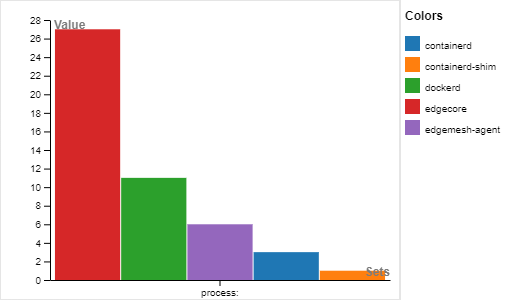
\includegraphics[width=\textwidth]{PICs/ke-cpu-noload.png}
        \caption{KubeEdge CPU without load}
    \end{minipage}
    %\hspace{.05\linewidth}
    \begin{minipage}[b]{.49\linewidth}
        \centering
        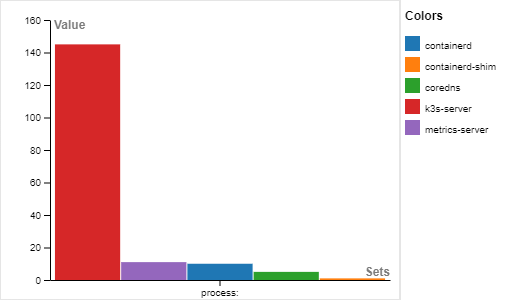
\includegraphics[width=\textwidth]{PICs/kf-cpu-noload.png}
        \caption{KubeFed CPU without load}
    \end{minipage}
    \label{fig:cpu-load-1}
\end{figure}
%https://app.rawgraphs.io/

In the diagram above, the process of cpustats itself and that of the SSH agent were not taken into account. Neither of them have any direct concern about the test performaed. Basically, the result can be interpreted in such a way that the load is low for both systems and no significant jumps were recognisable. Nevertheless, it must be noted that KubeEdge caused many times fewer CPU compared to KubeFed, while both system idle. The full CSV can be viewed in the designated folder on Github. The link is given at the end of the chapter.

\paragraph{Memory} Htop\cite{htop} and \ac{Aha}\cite{aha} were used to check the memory utilisation in idle mode. The measurement is carried out under the same conditions as the CPU test described above. The deployment was scaled to 1 on the corresponding node, no increased load must or had to be processed. The uptime of both system is 2 hours 15 minutes at time of testing. Since the memory behaves less erratically than the CPU, only one sample were taken. The total consumption for the both systems are:

\begin{itemize}
    \itemsep0em 
    \item \textit{KubeEdge} - 239 MB
    \item \textit{KubeFed} - 600 MB
\end{itemize}

The following table lists, in descending order, the 5 processes with the most RAM use and their percentage share of the total utilisation.

\begin{table}[ht]
    \begin{center}
        \begin{minipage}{.49\linewidth}
            \begin{center}
                \begin{tabular}{|l|l|}
                    \hline
                    Process & Usage in \%  \\
                    \hline
                    dockerd & 4,5 \\
                    edgecore & 4,2 \\
                    systemd-journald & 3,2 \\
                    edgemesh-agent & 2,6 \\
                    containerd & 2.2 \\
                    \hline
                \end{tabular}
                \caption{KubeEdge RAM uasge}
                \label{tab:ke-ram-noload}
            \end{center}
        \end{minipage}
        \begin{minipage}{.49\linewidth}
            \begin{center}
                \begin{tabular}{|l|l|}
                    \hline
                    Process & Usage in \%  \\
                    \hline
                    k3s & 24,0 \\
                    containerd & 6,9 \\
                    metrics-server & 2,4 \\
                    systemd-journald & 2,2 \\
                    coredns & 2.2 \\
                    \hline
                \end{tabular}
                \caption{KubeFed RAM uasge}
                \label{tab:kf-ram-noload}
            \end{center}
        \end{minipage}
    \end{center}
\end{table}
As the data shows, KubeEdge gets by with less RAM. KubeFed, on the other hand, uses almost three times as much. Although 600 MB may not seem like much in today's times, this can be important in some scenarios, especially in the context of edge-computing.

\paragraph{Disk} The last resource to be examined in this section is that of hard disk usage. The board tool "df" provided by Ubuntu shows the respective space allocated.

\begin{itemize}
    \itemsep0em 
    \item \textit{KubeEdge} - 3.5 GB allocated
    \item \textit{KubeFed} - 4.1 GB allocated
\end{itemize}
Similar to the results before, KubeEdge is also more efficient in this section.

\subsubsection{Load} In the next part of the tests-series, the behaviour during increased CPU and memory load is examined. Since we are only concentrating on the performance part of individual nodes and its effects in this section, no \ac{HPA} is used but only a pod that simulates high load. The behaviour of the overall system, when distributing and scaling application load is examinated in the \autoref{sec:dsrtestapp}. The same environment as for the previous tests is assumed as the basis for conducting the test. To test the described scenario, the tool "kube-stresscheck"\cite{kube-stress} is used. This tool creates a pod on one of the available edge-nodes which, on the one hand, occupies the entire \ac{RAM} and, on the other hand, utilises all available CPU cores.

It should be noted that the standard \ac{QoS} of \ac{K8s} is applied or maintained for system pods\cite{k8s-qos}. This mechanism provides three different levels of execution: Guaranteed, Burstable, BestEffort. As the name suggests, pods with the level guaranteed are assigned the highest priority. The test that is carried out is only assigned the level BestEffort and should therefore theoretically not be able to influence system pods that are assigned a higher level. In real operation, high loads can still cause considerable problems under certain circumstances. In productive settings, such tests should be refrained from.

\paragraph{KubeEdge} Due to the \ac{K8s} native support KubeEdge comes with, the configuration provided by kube-stresscheck is ready as is. The version selected is the one that only occupies one node with full load. In order to test the node that was selected as the input for the tests before, the other nodes are temporarily drained. Although the developers of the test application describe it as follows: "Usually pods like kube-proxy, nginx-ingress-controller, calico-node are crashlooping. If kubelet or docker was affected by stress test then node will become NotReady"\cite{kube-stress}. However, no such effects could be observed in the test run carried out. The following values were observed and recorded during the stress test on the affected node. 

\begin{itemize}
    \item \textit{Memory usage}: \textbf{100\%} - a flickering was noticed because the underlying \ac{OS} is trying to free-up unused allocated memory. On the other hand, the pod fills the \ac{RAM} directly again.
    \item \textit{CPU usage}: \textbf{100\%} throughout on both cpu cores during the test periode. 
\end{itemize}
The following behaviour was observed during the test, which was carried out over a period of one minute.

\begin{itemize} 
    \item \textit{Stability} - All functionalities of the environment were maintained during the test. Also all pods were available during the entire run and did not get re-scheduled or exited. All local services and agents at the edge-node also performed their services unhindered.
    \item \textit{Logs} - No errors could be read in the local logs of the respective nodes or in the kubernetes-specific logs. No indication of any problems that could be traced back to the load tests could be found within the test pods either.
    \item \textit{Responsiveness} - The test deployment responds and is fully available during the test period. The response times are somewhat slower, as described in the following \autoref{sec:dsrtestnetwork}.
    \item \textit{Recovery} - After the end of the test, operation was continue without any consequences. The CPU as well as RAM utilisation go back to the initial values. 
\end{itemize}
In summary, KubeEdge has done exceptionally well. No failures or noteworthy events were detected during the tests. Although the performance of the services that are located on the same node suffers, these effects were within limits and to some extent predictable. The effective use of \ac{QoS} could further improve overall performance.

\paragraph{KubeFed} The test is carried out under the same conditions as the test above. The test deployment is scaled to a pod on the target system, edge-1. However, since KubeFed does not offer an \ac{CNI} for intra-cluster service communication, the port is changed from ClusterIP to NodePort. This allows the connection test to be carried out using curl with the same conditions. The following values were observed and recorded during the stress test on the affected node.

\begin{itemize}
    \item \textit{Memory usage}: \textbf{100\%} - similar to the behaivor with KubeEdge, a flickering was noticed.
    \item \textit{CPU usage}: \textbf{100\%} throughout on both cpu cores during the test periode. 
\end{itemize}

The following behaviour was observed during the test, which was carried out over a period of one minute. With the exception of the response times, the same results were achieved. For the sake of completeness, these are listed again below.

\begin{itemize} 
    \item \textit{Stability} - All functionalities of the environment were maintained during the test. Also all pods were available during the entire run and did not get re-scheduled or exited. All local services and agents at the edge-node also performed their services unhindered.
    \item \textit{Logs} - No errors could be read in the local logs of the respective nodes or in the kubernetes-specific logs. No indication of any problems that could be traced back to the load tests could be found within the test pods either.
    \item \textit{Responsiveness} - Similar to the test before, the deployment of the test pod was reachable during the test. Details of this test, as mentioned earlier, can be found in the network-section in \autoref{sec:dsrtestnetwork}.
    \item \textit{Recovery} - After the end of the test, operation was continue without any consequences. The CPU as well as RAM utilisation go back to the initial values. 
\end{itemize}
In summary, KubeFed did also behaive very well during the tests. Even under heavy load, our test service performs well and only stands out due to slightly higher response times. As with KubeEdge, this could be further improved through the use of \ac{QoS}.

\subsubsection{Result and interpretation} 
Both systems can be considered resource efficient. KubeFed benefits from the use of K3s instead of vanilla K8s. Nevertheless, KubeEdge is the winner in terms of minimum requirements and may be preferable for edge locations with weak devices. Under high load, both environments could prove high stability.

\subsection{Network connectivity}
\label{sec:dsrtestnetwork}
\subsubsection{Reponse time}
In the course of the performance tests, which can be found in the \autoref{sec:dsrtestress}, network tests were also carried out to test the behaviour both under load and without load. For this purpose the tool curl is used which can measure time values via output parameters. The test-command is shown below.

\begin{lstlisting}[caption={Curl command},captionpos=b]
curl -w "@curl-output.txt" -o /dev/null -s IP:8000
\end{lstlisting}

The \hyperref{https://github.com/Berndinox/K8sEdge/blob/main/Tests/network/curl.md}{}{}{curl-output.txt} file defines the processing and output specifications. The call via curl is made from the respective master node located in Germany, as also shown in the following \autoref{tab:poc-nodes}. The target in each case is the node edge-1 which is hosted in the US and performs our target deployment. Due to the differences within the architecture of the two environments, different methods are used at this point. While the internal ClusterIP can be addressed for KubeEdge, which brings the data transfer to the target pod internally via EdgeMesh, a NodePort must be made accessible via the internet for KubeFed. This means that in the case of KubeFed, the curl command must be issued against the public IP of the target node. The service object of our usecase, describe in \autoref{sec:dsrusecase}, was therefore modified as follows for KubeFed.

\begin{lstlisting}[caption={Curl command},captionpos=b]
type: NodePort
ports:
- name: http
  port: 8000
  targetPort: 80
  NodePort: 30298
\end{lstlisting}

It should be noted that the default port-range for NodePorts is from 30000 to 32767.

\paragraph{KubeEdge} based on the command declared above, the following data could be obtained.

\begin{table}[ht]
    \begin{center}
        \begin{minipage}{.49\linewidth}
            \begin{center}
                \begin{tabular}{|l|l|}
                    \hline
                    Measuring point & Time \\
                    \hline
                    time\_namelookup & 0.000059s \\
                    time\_connect & 0.000581s \\
                    time\_pretransfer & 0.000663s \\
                    time\_starttransfer & 0.192938s \\
                    \hline
                    time\_total & 0.193011s \\
                    \hline
                \end{tabular}
                \caption{KubeEdge: curl no load (ClusterIP)}
                \label{tab:ke-con-noload}
            \end{center}
        \end{minipage}
        \begin{minipage}{.49\linewidth}
            \begin{center}
                \begin{tabular}{|l|l|}
                    \hline
                    Measuring point & Time \\
                    \hline
                    time\_namelookup & 0.000070s \\
                    time\_connect & 0.000245s \\
                    time\_pretransfer & 0.000316s \\
                    time\_starttransfer & 0.338320s \\
                    \hline
                    time\_total & 0.338480s \\
                    \hline
                \end{tabular}
                \caption{KubeEdge: curl with load (ClusterIP)}
                \label{tab:ke-con-load}
            \end{center}
        \end{minipage}
    \end{center}
\end{table}

The total time to complete a call increased by about 75\% in the test conducted. While this may sound like a large increase at first, it must be mentioned again that the node was under absolute full load. In this respect, this value is relativised and could even be considered quite good.

In order to provide a complete overview, although functions that constitute a decisive added value were deactivated, KubeEdge was also tested via HostPort. This variant is more comparable with the NodePort described above.

\begin{table}[ht]
    \begin{center}
        \begin{minipage}{.49\linewidth}
            \begin{center}
                \begin{tabular}{|l|l|}
                    \hline
                    Measuring point & Time \\
                    \hline
                    time\_namelookup & 0.000079s \\
                    time\_connect & 0.093761s \\
                    time\_pretransfer & 0.093832s \\
                    time\_starttransfer & 0.187626s \\
                    \hline
                    time\_total & 0.188056s \\
                    \hline
                \end{tabular}
                \caption{KubeEdge: curl no load (HostPort)}
                \label{tab:ke-con-noload-np}
            \end{center}
        \end{minipage}
        \begin{minipage}{.49\linewidth}
            \begin{center}
                \begin{tabular}{|l|l|}
                    \hline
                    Measuring point & Time \\
                    \hline
                    time\_namelookup & 0.000033s \\
                    time\_connect & 0.093475s \\
                    time\_pretransfer & 0.093552s \\
                    time\_starttransfer & 0.201756s \\
                    \hline
                    time\_total & 0.201889s \\
                    \hline
                \end{tabular}
                \caption{KubeEdge: curl with load (HostPort)}
                \label{tab:ke-con-load-np}
            \end{center}
        \end{minipage}
    \end{center}
\end{table}

The test via NodePort, which bypasses the internal network structure based on EdgeMesh, is similar to the following test of KubeFed. However, this variant also means that a decisive added value of KubeEdge is lost. This shows that EdgeMesh brings with it a certain overhead that should not go unnoticed.

\paragraph{KubeFed} under the same conditions, except for the adjustments to the service, the test was run through for KubeFed. The result is displayed below.

\begin{table}[ht]
    \begin{center}
        \begin{minipage}{.49\linewidth}
            \begin{center}
                \begin{tabular}{|l|l|}
                    \hline
                    Measuring point & Time \\
                    \hline
                    time\_namelookup & 0.000085s \\
                    time\_connect & 0.089800s \\
                    time\_pretransfer & 0.089906s \\
                    time\_starttransfer & 0.180030s \\
                    \hline
                    time\_total & 0.180333s \\
                    \hline
                \end{tabular}
                \caption{KubeFed: curl without load}
                \label{tab:kf-con-noload}
            \end{center}
        \end{minipage}
        \begin{minipage}{.49\linewidth}
            \begin{center}
                \begin{tabular}{|l|l|}
                    \hline
                    Measuring point & Time \\
                    \hline
                    time\_namelookup & 0.000042s \\
                    time\_connect & 0.089541s \\
                    time\_pretransfer & 0.089756s \\
                    time\_starttransfer & 0.225031s \\
                    \hline
                    time\_total & 0.225544s \\
                    \hline
                \end{tabular}
                \caption{KubeFed: curl with load}
                \label{tab:kf-con-load}
            \end{center}
        \end{minipage}
    \end{center}
\end{table}

The test only shows an increase of 25\%. Considering that the target node is under full load, this is an enormously good value and exceeds expectations. Especially under heavy load, Kubefed resp. a single target cluster, can process the request faster compared to KubeEdge and the EdgheMesh-agent.

\subsubsection{Connection restoring}
In addition to the ability to keep services available under heavy load, seamless restoration of availability is also important in the event of a disconnection. As with the previous runs, the test-deployment for this setup is scaled to a single pod on the node edge-1. The connection between the master and the node is then disconnected via the firewall function provided by Hetzner. This allows the connection to be cut without manipulating the nodes themselves. The following steps are then carried out in an orderly sequence for each environment.
\begin{enumerate}
    \itemsep0em
    \item Verify the availability of the pod via NodePort or HostPort
    \item Query the status of the node on the master
    \item Scaling of the test-deployment on the (unavailable) target node to two pods
    \item Restore the connection; disable the firewall rule
    \item Verify if the node is marked as available again without any action being taken
    \item Check if the deployment has been scaled accordingly
\end{enumerate}

During the entire run, any anomalies in the underlying system and within \ac{K8s} ecosystem are observed. The time until the system is fully restored and the deployment is scaled is also measured. Likewise, during disconnection, the service should continue to be available through HostPort for KubeEdge or NodePort in case of KubeFed. 




\subsubsection{Result and interpretation}

Latency Test, Offline Test
\subsection{Application stability}
\label{sec:dsrtestapp}
Caos Monkey

\section{Analysis}
\label{sec:dsranalysis}
\subsection{Relevant Magnitudes}
\subsection{Outcome}
\subsection{Paraphrase}



\chapter{Catalog}
\label{chap:catalog}

\section{Decision Variables}
\label{sec:variables}
\subsection{Installation complexity}
The first decision variable that is examined is the effort required for the installation and the associated complexity. According to the KISS principle\cite{kiss}, those solutions with less complexity should be preferred. One investigates the installation routine, descripted in the  \autoref{sec:dsrenv} "environment", very different steps and necessary tools were discovered. 
\paragraph{Dependencies} The first important variable we look at in this context are the dependencies. This paragraph considers requirements that must be met in order for the installation to proceed successfully.

\begin{itemize}
    \item \textit{Connectivity} - While KubeEdge works with literaly any connection when combined with EdgeMesh, even behind carrier-grade \ac{NAT}\cite{cg-nat}, important conditions must be checked for KubeFed, as descripted in \autoref{sec:dsrenvkf} under the paragraph "challenges". For the sake of completeness, the requirements for KubeFed are listed subsequent.
    \begin{itemize}
        \item Static \ac{IP} or dyn \ac{DNS} agent if dynamic assigned
        \item \ac{NAT} rule if the device is located behind a router
    \end{itemize}
    \item \textit{Device Support} - Both solutions offer a wide selection of different types of devices supported, like: ARM64, ARMv7, x86, or x64 based systems. However, because \ac{KubeFed} relies on a full functional \ac{K8s} cluster those extensive support is provided by the use of K3s and the container-runtime packaged within. In contrast, KubeEdge only requires on one of the supported container-runtimes as well as the KubeEdge binary. Because KubeEdge is taking special care of implementing lightweight agents compatible with \ac{CRI}\cite{k8scri}\cite{ke-cri-gh}, an even wider range of devices can be supported. Due to the design, even edge-devices with fewer resources can be used effectively. In summary, both solutions support a wide range of devices. KubeEdge, however, goes one step further and is therefore slightly in the lead.
    \item \textit{Other dependencies} - Other requirements such as bandwidth, connection quality and e.g. storage space have little or no influence on the installation itself and are therefore only considered in the following operational part.
\end{itemize}

\paragraph{Configuration} The second step is to examine the installation routine respectively the configuration steps itself.
\begin{itemize}
    \item \textit{Required Tools} - One important part is the number of tools and binaries used respectivley required to be able to run the environments. The fewer components are used, the less complex the installation and operation. The fewer components used, the greater the tendency to keep the environment simple. Although individual components can also involve quite a high degree of complexity, this variable must not be disregarded. The individual configuration steps are evaluated in the following sections. All tools are listed for each environment subsequent.
    \begin{itemize} 
        \item \textit{KubeEdge}
        \begin{itemize}
            \item \ac{CRI} (e.g. Docker)
            \item KubeEdge binaries
            \item K3s (Master only)
            \item EdgeMesh (Master only)
        \end{itemize}
        \item \textit{KubeFed}
        \begin{itemize}
            \item K3s
            \item KubeFed binaries (Master only)
            \item Helm (Master only)
        \end{itemize}
    \end{itemize}
    It should be noted that K3s includes or builds on \ac{CRI}. 
    \item \textit{Configuration steps} - This property describes the necessary steps that were required during the installation without additional tools. For KubeEdge the basic installation, without any logging capability and a working \ac{CNI}, is done by using a single binary. However, if logging is necessary (in almost all cases it should be), some adaptations must be made. The same applies to the installation of EdgeMesh, as described in \autoref{sec:dsrusecaseweb}. As the documentation is not clear enough, increased complexity and the associated effort are to be expected. For Kubefed, in contrast, the respective kubeconfig must be transferred to the master and added there as a custom context. This context is then added via kubefed binary. If one only examines the steps that are necessary to operate the two architectures in a meaningful way, these are much easier to accomplish for KubeFed. On the other hand, KubeEdge requires additional configurations and tools to be installed in order to be able to use the full range of functions. If you are looking for a simple and straightforward solution, KubeFed is the  winner in this section.
    \item \textit{Documentation}  - Both documentations appear well maintained and kept up to date. The KubeEdge updates seem a little more recent according to the Github history. The KubeFed documentation can only be read in the form of markdown files within Github, but there is a separate web page for KubeEdge. It must be noted, however, that the part concerning network and connectivity is unclear or not sufficiently described. After research, the extension EdgeMesh, which offers its own documentation, could be found. However, the interaction between the components KubeEdge or the Autonomic Kube-API Endpoint, the MetaManager and EdgMesh is insufficiently described. Overall, therefore, the KubeFed documentation is easier to read and understand.
\end{itemize}

\paragraph{Summarised assessment} The following table presents the above facts in a clear form.  
\begin{table}[ht]
    \begin{center}
        \begin{tabular}{|l|l|l|l|l|}
            \hline
            Category & Criteria & Property & \textbf{KubeEdge} & \textbf{KubeFed} \\
            \hline
            dependency & connectivity  & w/o static \ac{IP} & \cmark & \xmark \\
            dependency & connectivity  & w/o dNAT & \cmark & \xmark \\
            dependency & device support & extensive support & \cmark & \cmark \\
            dependency & device support & ressources efficiency & \textbf{high} & \textbf{moderate} 
            \\
            configuration & required tools & master/edge & \textbf{4/2} & \textbf{4/2} \\
            configuration & handling & necessary effort & \textbf{high} & \textbf{moderate} \\
            configuration & documentation & clarity/actuality & \textbf{moderate} & \textbf{good} \\
            \hline
        \end{tabular}
        \caption{Installation complexitiy overview}
        \label{tab:install-overview}
    \end{center}
\end{table}

\subsection{Community and support}
Another important factor is the support and the community for the respective application. Especially with relatively new and intuitive software, it is important to either have access to the community to exchange ideas and discuss problems, or to have a manufacturer who can provide support if needed. This is even more true if you want to use the environment productively and commercially.

\paragraph{Community} Both products offer an active community with regular meetings, an mailing list and Slack channel. The open source approach promotes the formation of these open communities. KubeEdge is somewhat more active in research than KubeFed, but this does not necessarily mean that you will be better with one or the other.

\paragraph{Support} At time of writing, we could not find any official company offering commercial support for the products. This is also, as mentioned above, due to the opensource approach. For KubeEdge, however, there is a list of companies that already use the product and support it accordingly. Among them are well-known companies such as Huawei, Orange and ARM. For KubeFed such a list is not disclosed. In compensation, the project is managed by Jeremy Olmsted-Thompson (Google) and Paul Morie (Apple) for this purpose. For both projects, issues can be submitted via Github.

\paragraph{Activity} During the investigation of the topic, KubeEdge seems to be a bit more in the hype than KubeFed. This indirectly also leads to getting the necessary support faster. Details on the topicality can be found in the next subsection "future proof".

\paragraph{Summarised assessment} The properties revealed above are tabulated below.  
\begin{table}[ht]
    \begin{center}
        \begin{tabular}{|l|l|l|l|l|}
            \hline
            Category & Criteria & Property & \textbf{KubeEdge} & \textbf{KubeFed} \\
            \hline
            community & communication-channel  & Slack & \cmark & \cmark \\
            community & communication-channel  & mailing-list & \cmark & \cmark \\
            community & communication-channel & regular meeting & \cmark & \cmark \\
            support & commercial & maintenance & \xmark & \xmark \\
            support & non-commercial & Github issues & \cmark & \cmark \\
            support & sponsors & official list & \cmark & \xmark \\
            activity & hype & movement & \textbf{high} & \textbf{medium} \\
            \hline
        \end{tabular}
        \caption{Community and support overview}
        \label{tab:cs-overview}
    \end{center}
\end{table}

\subsection{Future proof}
Another important element when deciding between the two options is how promising each is for the future. Especially, as in our case, when the project is mainly supported and developed by the community. In the following, the background of the projects, the topicality of the software updates as well as the media impact will be examined. The companies that use or support the project also play an important role in this context.

\paragraph{Releases} An important factor are the release cycles and the associated update frequency. An overview of all versions and updates can be found in the "Releases" site of each Github project. Both projects offer new versions on a regular basis, but KubeEde has slightly shorter cycles. Since the beginning of the year (2022), KubeEde has released two versions and KubeEdge has released one \cite{ke-releases-gh}\cite{kf-releases-gh}. The difference is only small at this point, both products shine with topicality.

\paragraph{Github Stats} Other characteristics that can define the future viability are the current stats from Github. The following table compares the two projects.

\begin{table}[ht]
    \begin{center}
        \begin{tabular}{|l|l|l|}
            \hline
            Github Stat & \textbf{KubeEdge} & \textbf{KubeFed} \\
            \hline
            Stars & 4800 & 2100 \\
            Forks & 1300 & 470 \\
            Releases & 30 & 32 \\
            Contributers & 229 & 87 \\
            Open issues & 147 & 23 \\
            Open pull-requests & 34 & 8 \\
            \hline
        \end{tabular}
        \caption{Github stats overview}
        \label{tab:gh-stats}
    \end{center}
\end{table}

It should be noted that the table shown above is only a snapshot. The values may change accordingly. It must also be noted that the higher number of reported problems may also result from more frequent use. Therefore, the correct interpretation is important.

\paragraph{Membership} KubeEdge is listed as a \ac{CNCF} project in the incubation phase. \ac{CNCF} is a central home for the fastest growing projects in the cloud native category. Even \ac{K8s} itself was part of it. In contrast, KubeFed is supported and further developed by the \ac{K8s} oriented \ac{SIG}. It stands out that due to the group membership clear rules concerning the further development have to be observed.

\paragraph{Sponsors} As already mentioned in section "community and support", KubeEdge is officially sponsored by some well-known companies. It should be noted, however, that these are mainly Chinese companies.

\paragraph{Independencie} A final important characteristic with regard to future-proofing is the extent to which a solution can be used without further development of the respective application. Although this assumption represents a worst-case scenario that seems rather unlikely in the foreseeable future, it should nevertheless be taken into account. KubeEdge uses a completely self-developed solution on the worker nodes. To replace it, all nodes must be reinstalled with the vanilla component of \ac{K8s}. Besides the effort involved, important functions concerning edge-computing are lost. \ac{KubeFed} offers a better solution here, due to its different architecture. Each node on the edge is a complete and independent worker. If KubeFed is no longer used, applications continue to run for the time being; no new installation is necessary on the nodes. The control could be taken over by alternative approaches, e.g. via \ac{CI/CD} pipelines. KubeFed thus offers better independence.

\paragraph{Summarised assessment} The characteristics relating to future viability are summarised below.  
\begin{table}[ht]
    \begin{center}
        \begin{tabular}{|l|l|l|l|l|}
            \hline
            Category & Criteria & Property & \textbf{KubeEdge} & \textbf{KubeFed} \\
            \hline
            future-proof & releases  & frequency & \textbf{very-high} & \textbf{high} \\
            future-proof & Github  & stars & \textbf{5k} & \textbf{2k} \\
            future-proof & Github & activities & \textbf{high} & \textbf{moderate} \\
            future-proof & membership & development programm & \textbf{CNCF} & \textbf{SIG} \\
            future-proof & sponsors & companies & \cmark & \xmark \\
            future-proof & independencie & alternative option & \xmark & \cmark \\
            \hline
        \end{tabular}
        \caption{future-proof overview}
        \label{tab:fp-overview}
    \end{center}
\end{table}

\section{Criteria catalogue}
\label{sec:cc}
The following catalogue of criteria can be compiled on the basis of the data obtained in \autoref{sec:variables}. Zangemeister defines the method as follows: "Utility analysis is the analysis of a set of complex alternative actions with the purpose of ordering the elements of this set according to the preferences of the decision maker with respect to a multidimensional goal system"\cite{nwa}. By awarding points for each sub-area, the target environment with the highest effectiveness can be selected. The multiattribute value function is used for this purpose. The sum of the calculated individual attributes results in the total value per solution.

\begin{equation*}
v(a) = \sum \limits_{r=0}^{m}w_{r} v_{r} (a_{r})
\end{equation*}

w(r) must be greater than 0 and the condition of validity of the value function must be fulfilled.

\begin{equation*}
\sum \limits_{r=0}^{m} w_{r} = 1
\end{equation*}

Provided that the above mathematical principles are followed, individual weightings can be assigned. This achieves a high degree of flexibility of the catalogue. 

\subsection{Table}
The following table acts as a criteria catalogue. Based on the previous qualitative research using the \ac{DSR} method, the values were obtained. Due to the many different areas of application or objectives that are targeted, this table can be adapted according to one's own requirements.However, the values given serve as orientation points or generalised starting values. There is an empty table in the \autoref{appendix} that serves as a template so that adjustments can be made easily.

\begin{table}[ht]
    \begin{center}
        \resizebox{\textwidth}{!}{\begin{tabular}{|l|l|l|l|l|l|l|l|}
            \hline
            \multicolumn{2}{|l|}{Category} & \multicolumn{2}{l|}{Criteria} & \multicolumn{2}{l|}{Rating} & \multicolumn{2}{l|}{Weighted rating} \\
            \hline
            Name & Weight & Criteria & Weight & KubeEdge & KubeFed & KubeEdge & KubeFed \\
            \hline
            Installation & 30\% & connectivity & 10\% & 5 & 1 & 0,5 & 0,1 \\
            & & device support & 10\% & 5 & 4 & 0,5 & 0,4 \\
            & & required tools & 2\% & 3 & 3 & 0,06 & 0,06 \\
            & & configuration & 2\% & 2 & 4 & 0,04 & 0,08 \\
            & & documentation & 6\% & 2 & 4 & 0,12 & 0,24 \\
            \hline
            Commuity & 6\% & communication channels & 3\% & 5 & 5 & 0,15 & 0,15 \\
            & & actual hype & 3\% & 4 & 3 & 0,12 & 0,09 \\
            \hline
            Support & 10\% & commercial maintenance & 5\% & 0 & 0 & 0 & 0 \\
            & & bug reporting & 4\% & 5 & 5 & 0,2 & 0,2 \\
            & & sponsor-list & 1\% & 5 & 0 & 0,05 & 0 \\
            \hline
            Future-proof & 10\% & Github stats & 3\% & 4 & 3 & 0,12 & 0,09 \\
            & & release cycles & 3\% & 4 & 3 & 0,12 & 0,09 \\
            & & independencie & 3\% & 1 & 4 & 0,03 & 0,09 \\
            & & commercial sponsors & 1\% & 5 & 0 & 0,05 & 0 \\
            \hline
        \end{tabular}}
        \caption{Criteria catalog table}
        \label{tab:cct}
    \end{center}
\end{table}
To define your own values, proceed as follows. First, the categories are given the appropriate weighting. The total value of all categories must amount to 100\%. The more important a category is or is to be included in the evaluation, the higher the percentage value assigned should be. Then the percentage value of a category is divided into the criteria below it. So if the category is rated 20\%, two criteria can be assigned 10\% each, for example. The next step is to evaluate the respective criteria for the two environments. The pre-filled values above serve as an initial value respectively approximation. A value between 1 (low, bad) and 5 (high, good) is indicated. The weight is then calculated using the following formula.

\begin{equation*}
    \frac{CriteriaWeight}{100}*Rating
\end{equation*}

The permitted value range for the rating must be taken into account.
\begin{equation*}
    Rating = \left\{1,2,3,4,5  \right\}
\end{equation*}

\section{Exclusions and Special Cases}
\label{sec:exclusions}
TODO: If somethin is really a requirement. How to mark it at the catalog?



\chapter{Related Work}
\label{chap:related}
\section{Kubernetes and the Edge?}
Some introdution to K8s at the Edge, highlighting the main Architectures.
\section{Extend Cloud to Edge with KubeEdge}
Descripes KubeEdge and its advantages
\section{Sharpening Kubernetes for the Edge}
Sharpening Kubernetes for the Edge
Make Kubernetes aware of the latency between the nodes at the Edge.
\section{Ultra-Reliable and Low-Latency Computing in the Edge with Kubernetes}
Similar to the paper before. Latecny awar pod deploymentm, but you also can deploy to regions and an custom re-scheduler is implementated taking care of redeploying when one node fails.
Clustering node-groups based on latency.


\chapter{Results}
\label{chap:results}

\section{Findings}
\label{sec:findings}

\section{Conclusio}
\label{sec:conclusio}

\section{Discussion and further research}
\label{sec:discuss}
Combine KubeEdge and KubeFed (distributed hybrid Kubernetes)



%
% Hier beginnen die Verzeichnisse.
%
\clearpage
%\ifthenelse{\equal{\FHTWCitationType}{HARVARD}}{}{\bibliographystyle{biblatex}}
%\bibliography{Literatur}
\printbibliography 
\clearpage

% Das Abbildungsverzeichnis
\listoffigures
\clearpage

% Das Tabellenverzeichnis
\listoftables
\clearpage

% Das Quellcodeverzeichnis
\listofcode
\clearpage

\phantomsection
\addcontentsline{toc}{chapter}{\listacroname}
\chapter*{\listacroname}
\begin{acronym}[XXXXX]
    \acro{IT}[IT]{information technology}
    \acro{WWW}[WWW]{world wide web}
    \acro{K8s}[K8s]{Kubernetes}
    \acro{IoT}[IoT]{internet-of-things}
    \acro{DSR}[DSR]{design science research}
    \acro{CLI}[CLI]{command line interface}
    \acro{QoS}[QoS]{quality of service}
    \acro{CPU}[CPU]{central processing unit}
    \acro{RAM}[RAM]{random access memory}
    \acro{CNI}[CNI]{container network interface}
    \acro{IP}[IP]{internet procotcol}
    \acro{NAT}[NAT]{network address translation}
    \acro{DNS}[DNS]{domain name system}
    \acro{MQTT}[MQTT]{message queuing telemetry transport}
    \acro{CNCF}[CNCF]{Cloud Native Computing Foundation}
    \acro{KubeFed}[KubeFed]{Kubernetes cluster federation}
    \acro{API}[API]{application programming interface}
    \acro{PoC}[PoC]{proof-of-concept}
    \acro{ARM}[ARM]{advanced RISC machines}
    \acro{OS}[OS]{operating system}
    \acro{GUI}[GUI]{graphical user interface}
    \acro{VPN}[VPN]{virtual private network}
    \acro{FQDN}[FQDN]{full qualified domain name}
    \acro{CRI}[CRI]{container runtime interface}
    \acro{SIG}[SIG]{special interessts group}
    \acro{CI/CD}[CI/CD]{continuous integration / continuous delivery}
    \acro{CRD}[CRD]{costum ressource definition}
    \acro{HPA}[HPA]{horizontal pod autoscaler}
    \acro{Aha}[Aha]{Ansi HTML adapter}
\end{acronym}

%
% Hier beginnt der Anhang.
%
\clearpage
\appendix
\chapter{Appendix}
\label{appendix}
\end{document}